\documentclass{lug}
\usepackage{graphicx}
\usepackage{amsmath}
\usepackage{bm}
\usepackage{color}
\def\code#1{\texttt{#1}}

\title{Neural Acceleration for General-Purpose Approximate Programs}
\author{Hadi Esmaeilzadeh, Adrian Sampson, Luis Ceze and Doug Burger}
\institute{\textbf{Presented By:} \\ Lou Brand \\ Department of Computer Science\\Colorado School of Mines}
\date{\today}

\begin{document}

\section{Motivation}

\frame{
    \frametitle{Efficiency vs. Programmability}
    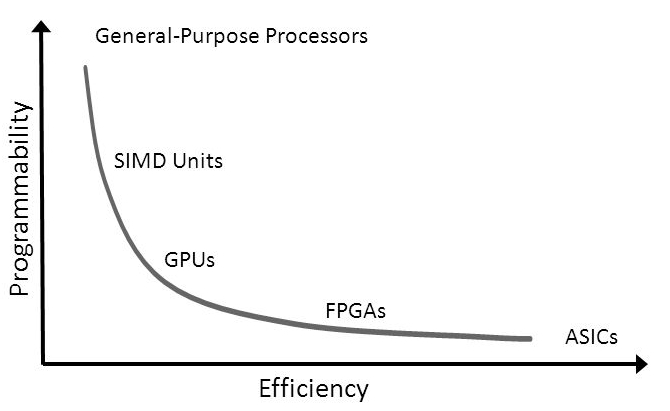
\includegraphics[scale=.60]{images/programmability-vs-efficiency.jpg} 
}

\frame{
    \frametitle{Challenges}
    \begin{itemize}[<+->]
        \item \textbf{Learning Algorithm:} Finding an algorithm that can accurately and efficiently mimic (approximate) imperative code
        \item \textbf{Language Compilation Framework:} Develop a programming model to transform existing code
        \item \textbf{Architectural Interface:} Low overhead hardware implementation
    \end{itemize}
}

\section{Approach}
\frame{
    \frametitle{The Parrot Transformation}
    \center{
        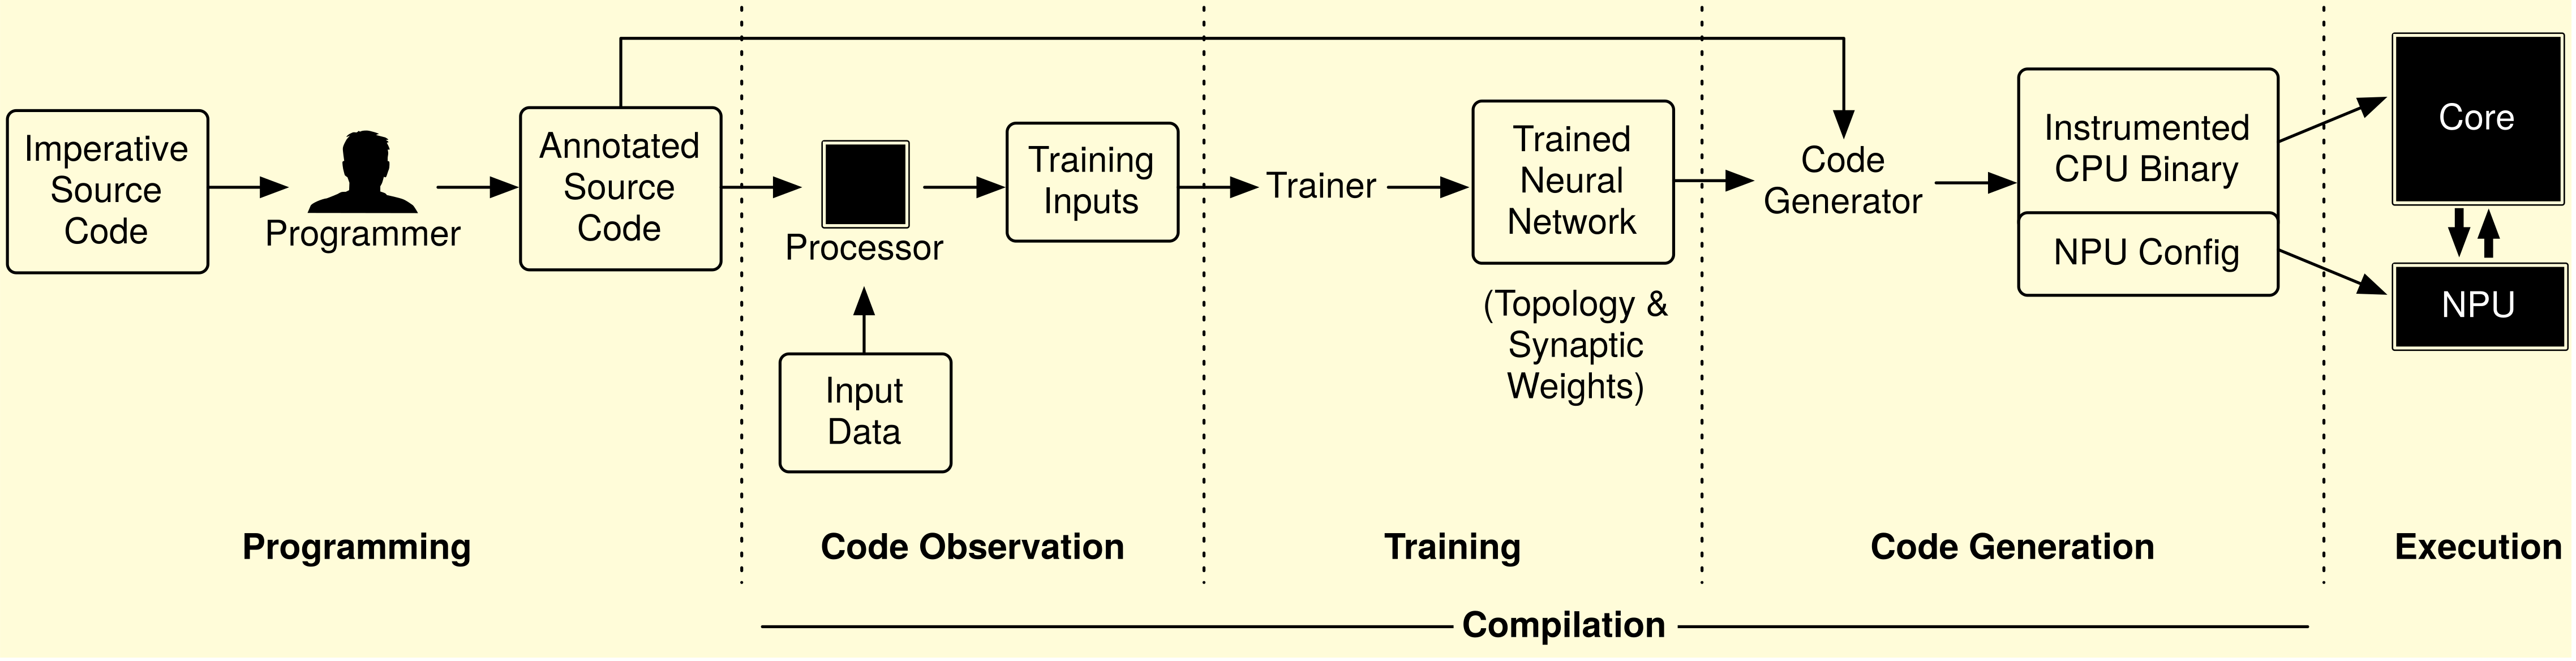
\includegraphics[scale=.6]{images/fig1.png}
    }
    \begin{enumerate}[<+->]
        \item \textbf{Programming:} Programmer explicitly labels functions that can be approximated
        \item \textbf{Code Observation:} Compiler records inputs/outputs of annotated code
        \item \textbf{Training:} Trains neural network that mimics code regions
        \item \textbf{Code Generation:} Generate code for the Neural Processing Unit (NPU)
        \item \textbf{Execution:} NPU is invoked for programmer defined section 
    \end{enumerate}
}

\frame{
    \frametitle{Code Annotation}
    \center{
        
\includegraphics[scale=1.0]{images/fig2a.png}\\
        \textbf{Key:} inputs/outputs must be defined at compile time
   }
}

\frame{
    \frametitle{Code Annotation}
    \center{
        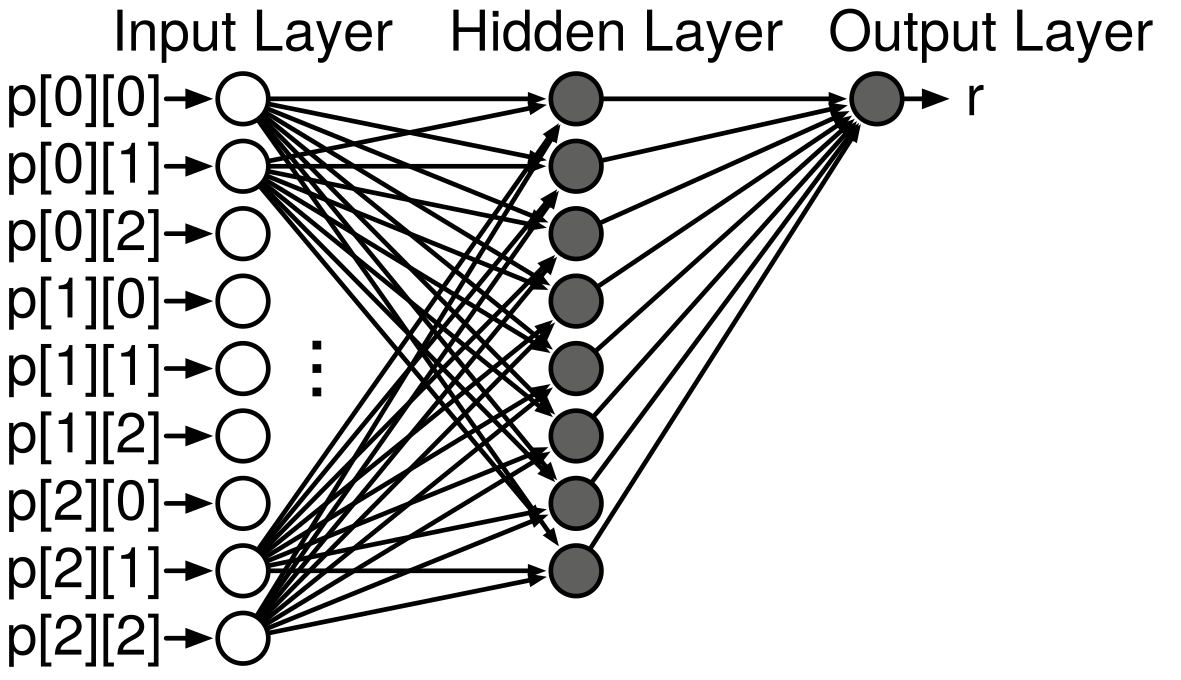
\includegraphics[scale=1.0]{images/fig2b.png}\\ 
        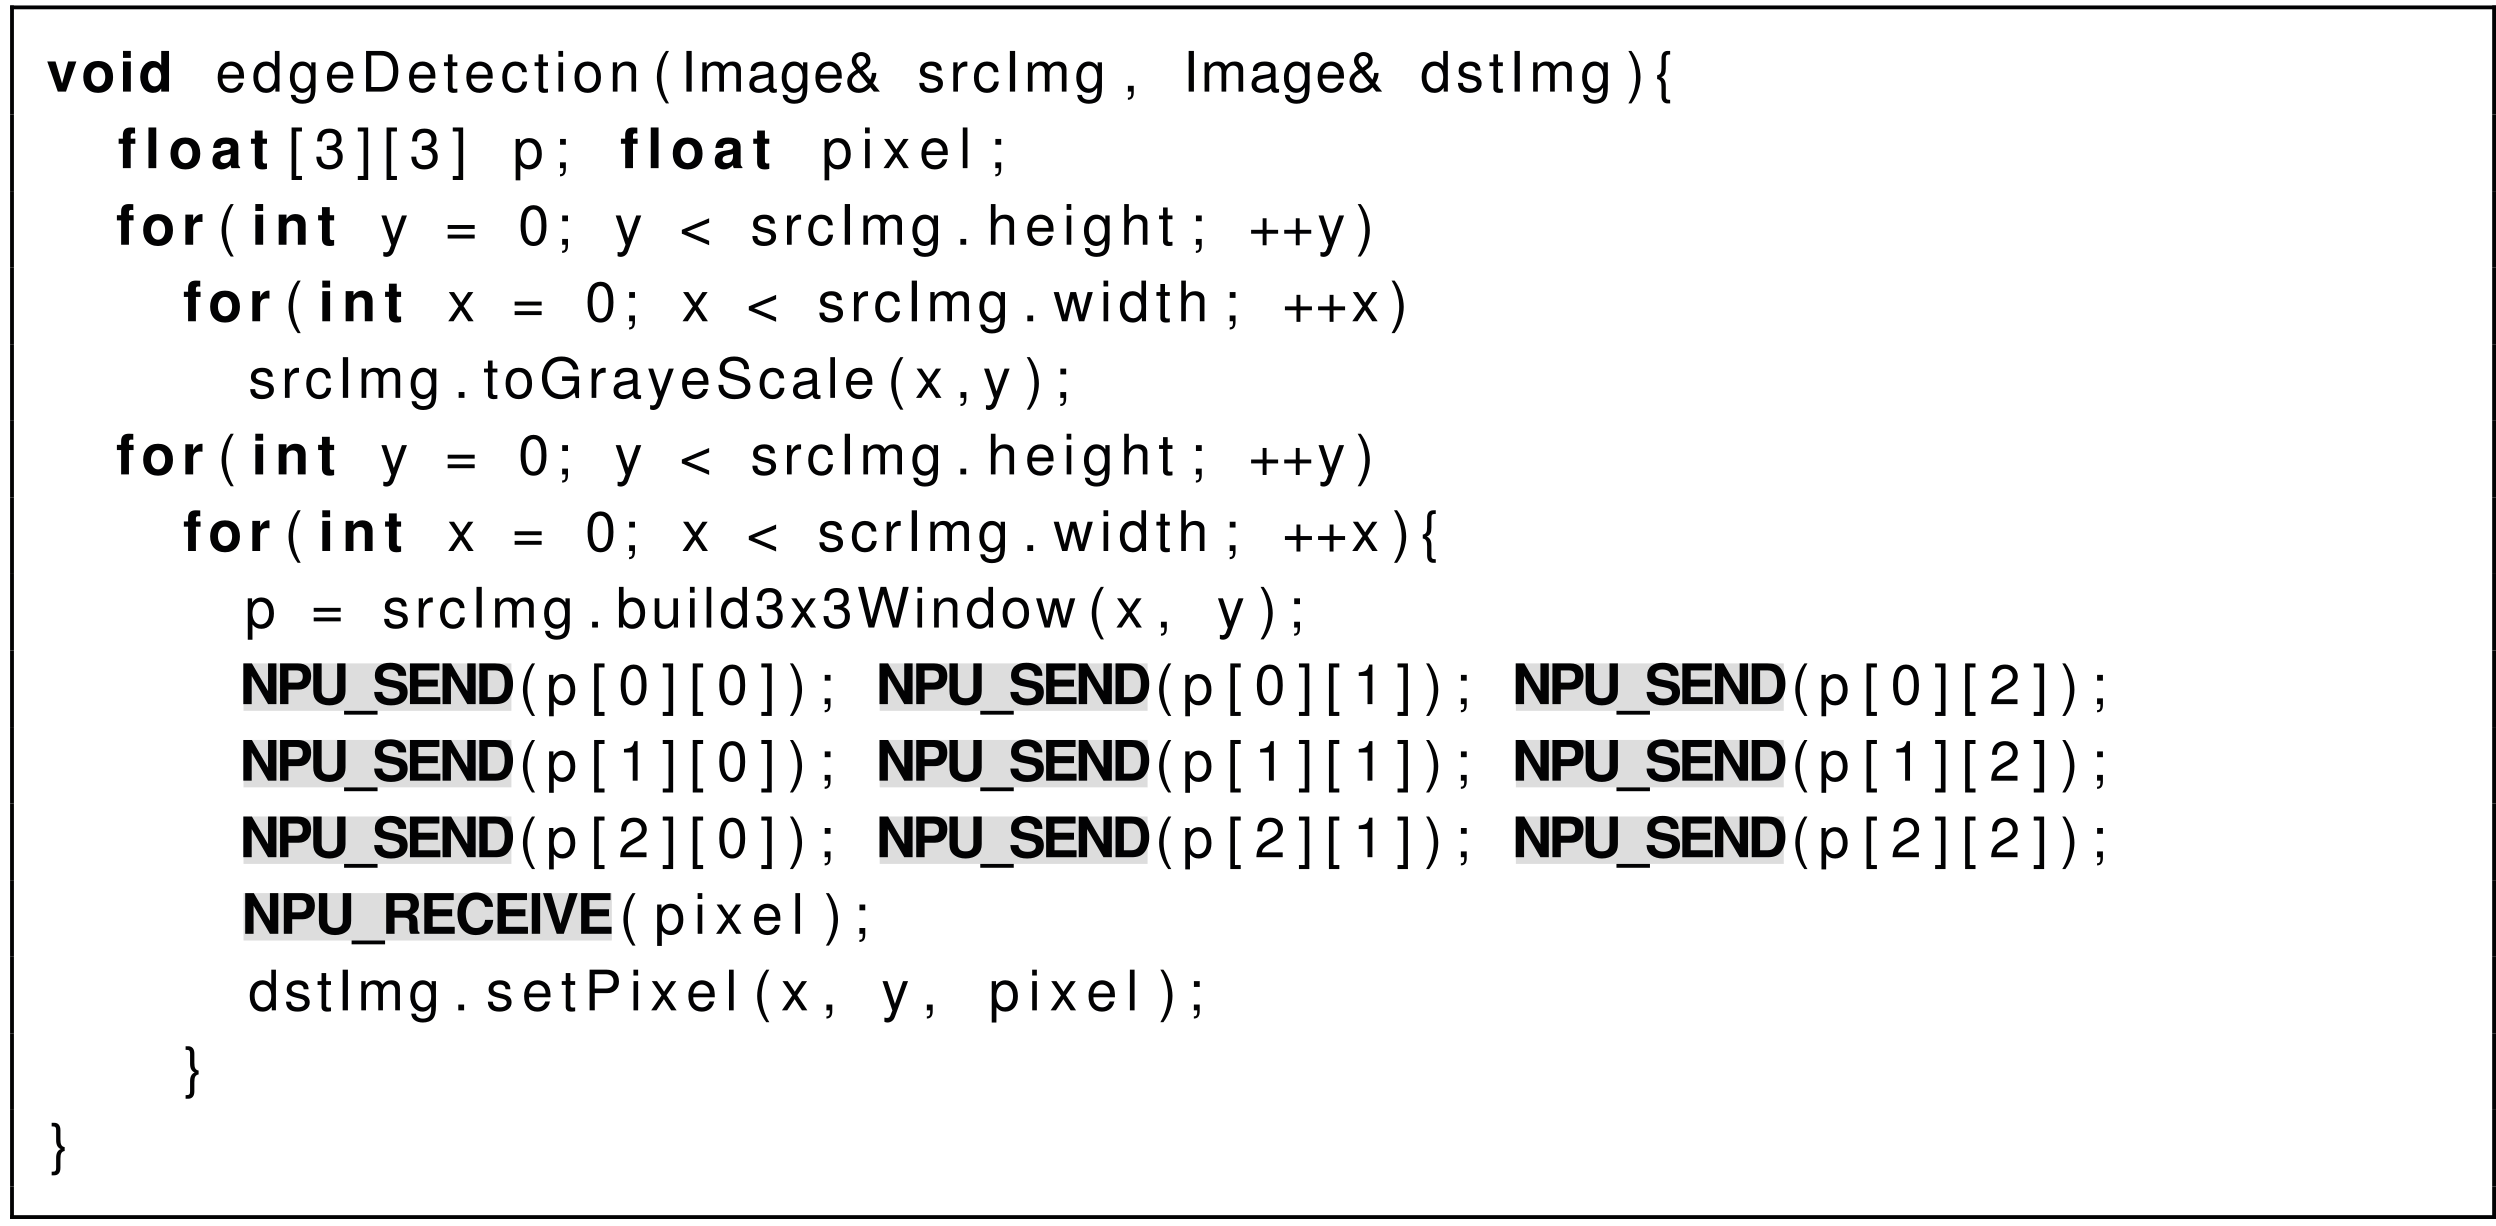
\includegraphics[scale=1.0]{images/fig2c.png}\\
        \textbf{Key:} inputs/outputs must be defined at compile time
    }
}

\frame{
    \frametitle{Neural Processing Unit (NPU)}
    \center{
        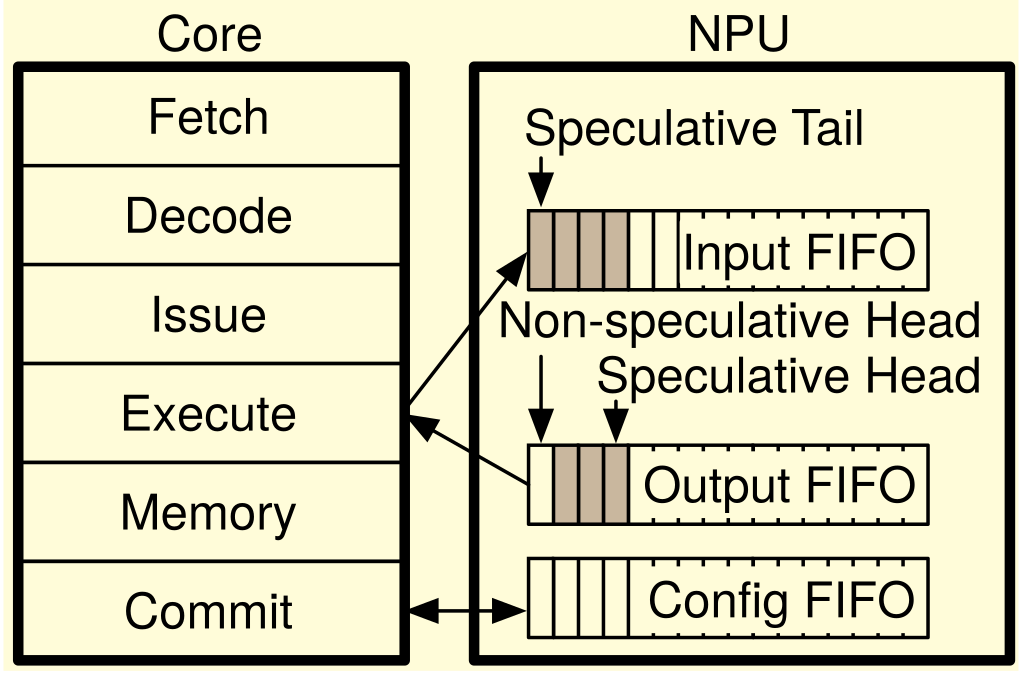
\includegraphics[scale=1.0]{images/fig3.png}\\
    }
    \begin{itemize}[<+->]
        \item \textbf{enq.c \%r:} enqueues value of register r into config FIFO 
        \item \textbf{deq.c \%r:} dequeues a configuration value from config FIFO to register r
        \item \textbf{enq.d \%r:} enqueues value of register r into input FIFO 
        \item \textbf{deq.d \%r:} dequeues the head of the output FIFO to register r  
    \end{itemize}
}

\frame{
    \frametitle{Reconfigurable NPU}
    \center{
        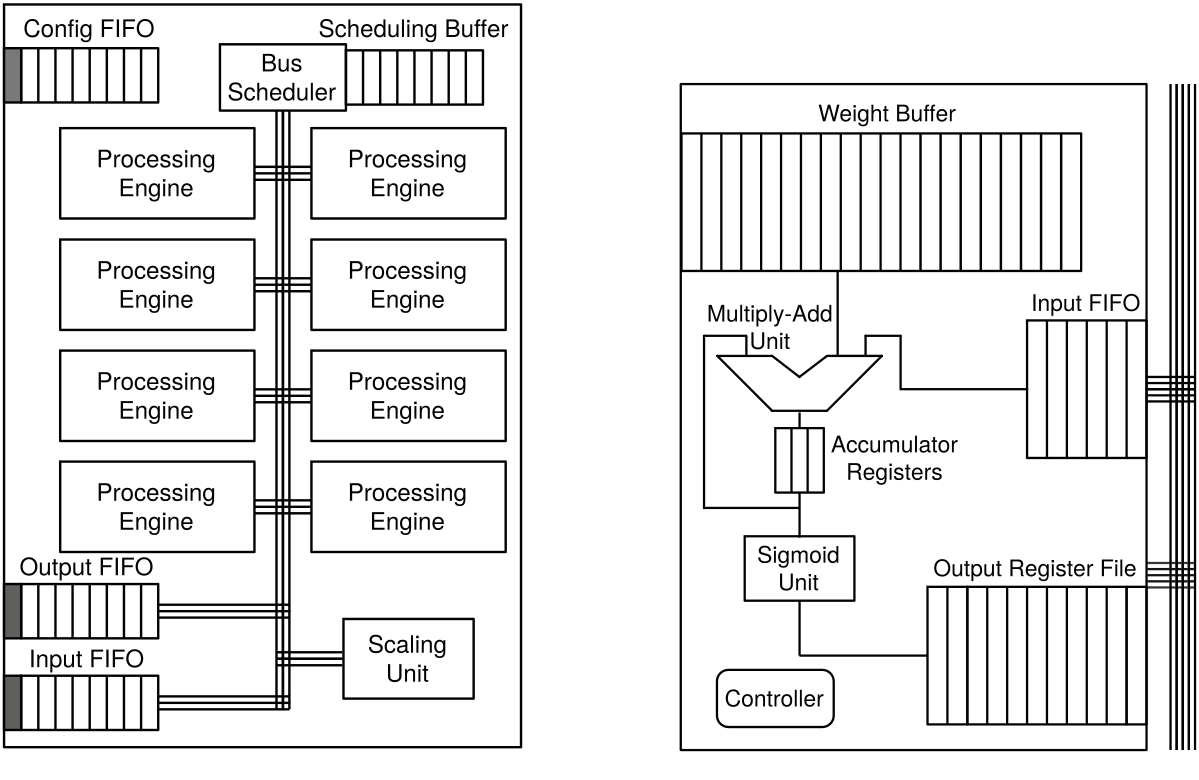
\includegraphics[scale=1.0]{images/fig5.png}\\
        Configured During Code Generation
    }
}

\section{Experiments}
\frame{
    \frametitle{Benchmarks}
    \begin{itemize}[<+->]
        \item \textbf{Signal Processing:} \code{fft} 
        \item \textbf{Robotics:} \code{inversek2j} 
        \item \textbf{3D Gaming:} \code{jmeint}
        \item \textbf{Compression:} \code{jpeg}
        \item \textbf{Machine Learning:} \code{kmeans}
        \item \textbf{Image Processing} \code{sobel} 
    \end{itemize}
    \center{
        \pause
        \textbf{Goal:} Illustrate versatility for the Parrot Transformation\\
        \pause
        \textbf{Note:} Each application has a different NPU configuration\\
        \pause
    }
}

\frame{
    \frametitle{Approximation Evaluation}
    \center{
        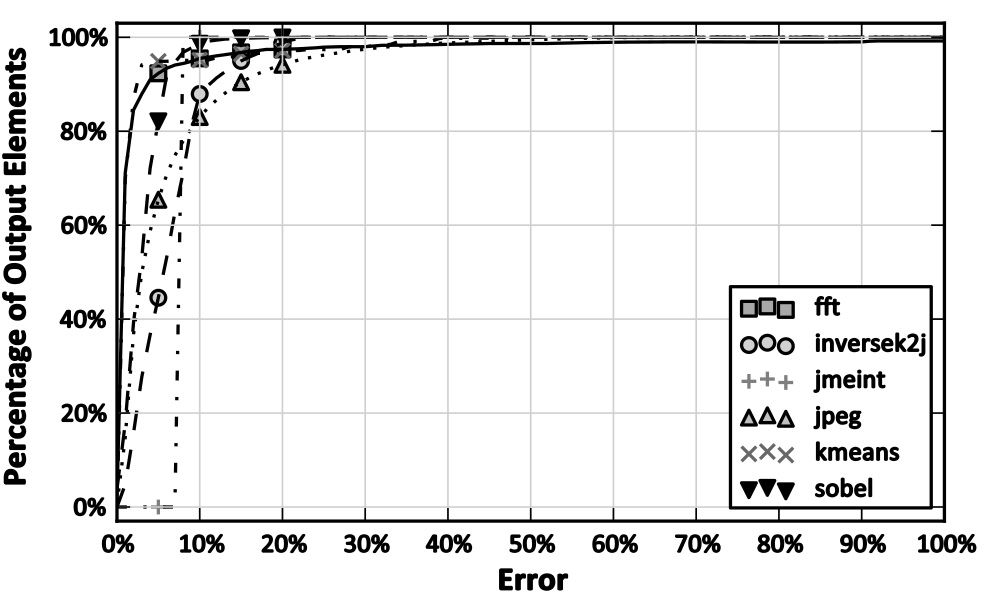
\includegraphics[scale=1.0]{images/fig6.png}\\
        Majority of output approximations, using the Parrot Transformation, show less than 10\% error. 
    }
}

\frame{
    \frametitle{Dynamic Instruction Count}
    \center{
        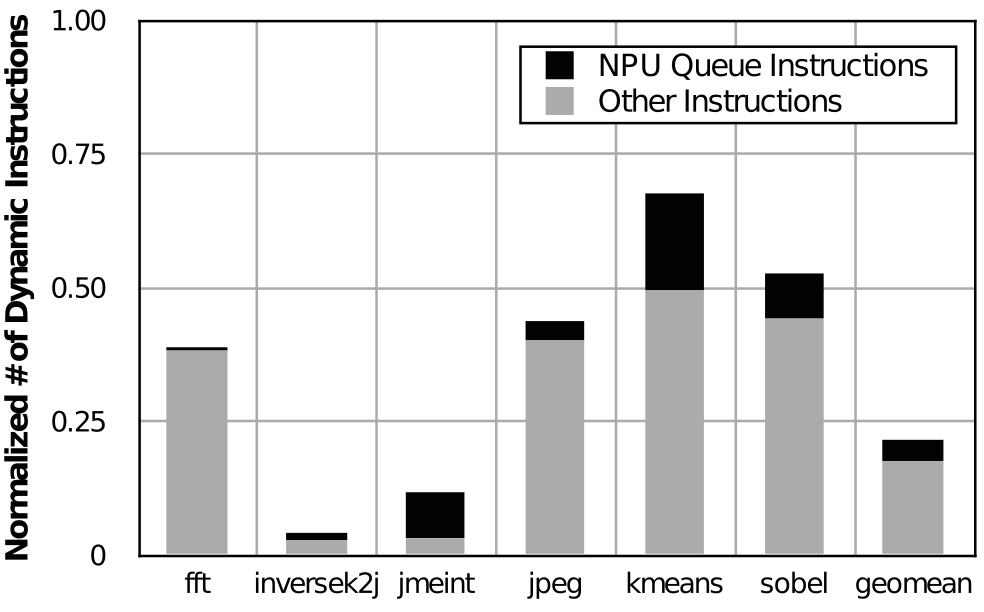
\includegraphics[scale=1.0]{images/fig7.png}\\
        \textbf{Insight:} Potential benefit of NPU acceleration is directly related to amount of CPU work it can replace... Sound familiar? \\
        \setbeamercovered{invisible}
        \pause \textbf{Amdahl's Law}
        \setbeamercovered{transparent}
    }
}

\frame{
    \frametitle{Speedup (NPU)}
    \center{
        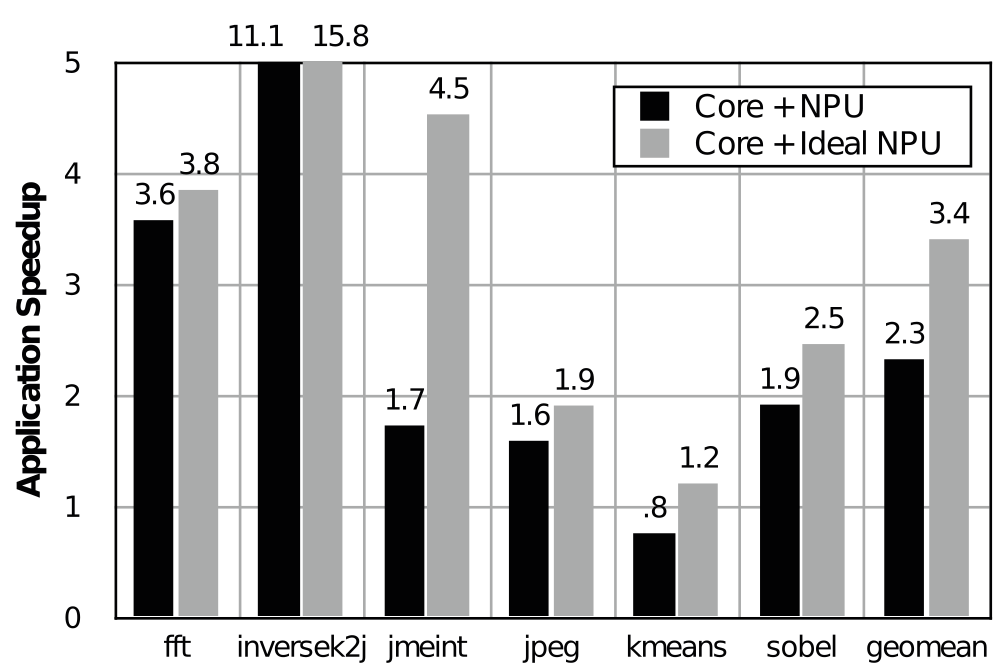
\includegraphics[scale=1.0]{images/fig8a.png}\\
        Average NPU acceleration: 2.3$\times$ speedup
    }
}

\frame{
    \frametitle{Slowdown (FANN)}
    \center{
        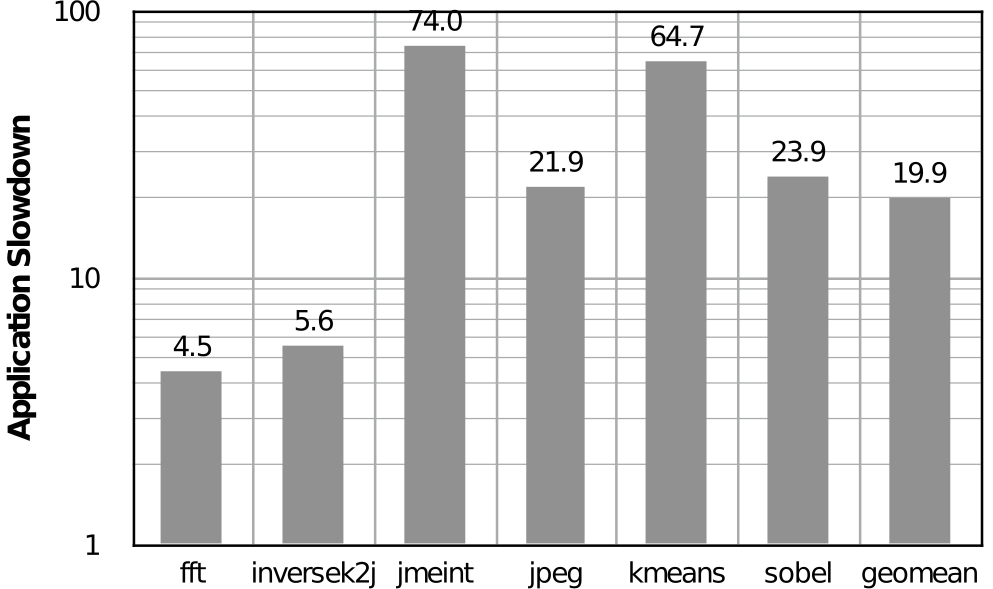
\includegraphics[scale=1.0]{images/fig9.png}\\
        Hardware implementation of the NPU is a \textbf{vital component}. 
    }
}

\frame{
    \frametitle{Energy Reduction}
    \center{
        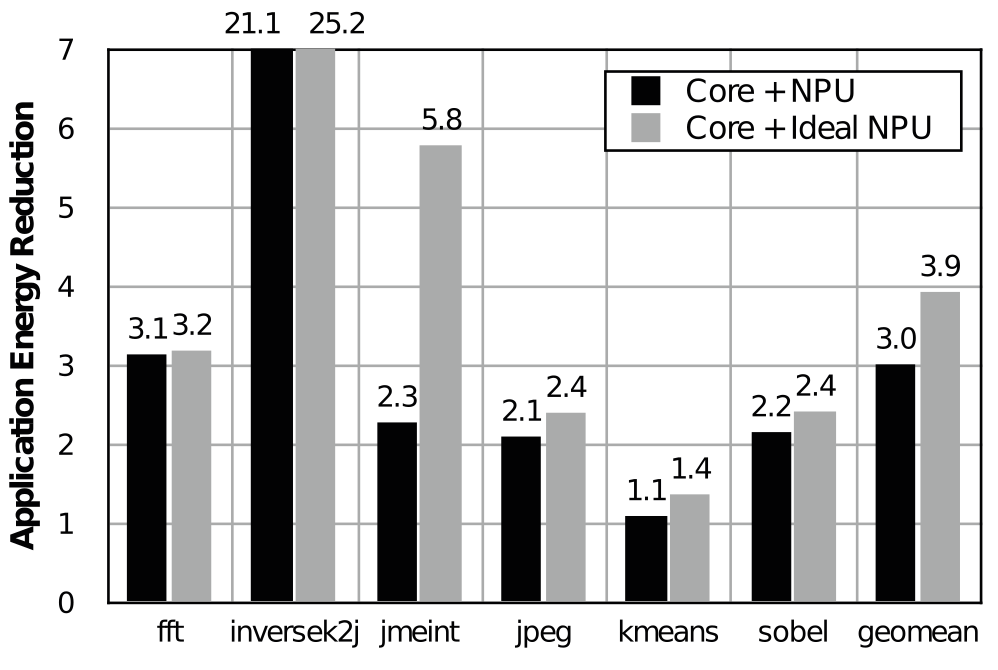
\includegraphics[scale=1.0]{images/fig8b.png}\\
        Average NPU power savings: 3.0$\times$ energy reduction
    }
}

\frame{
    \frametitle{Sensitivity to Communication Latency}
    \center{
        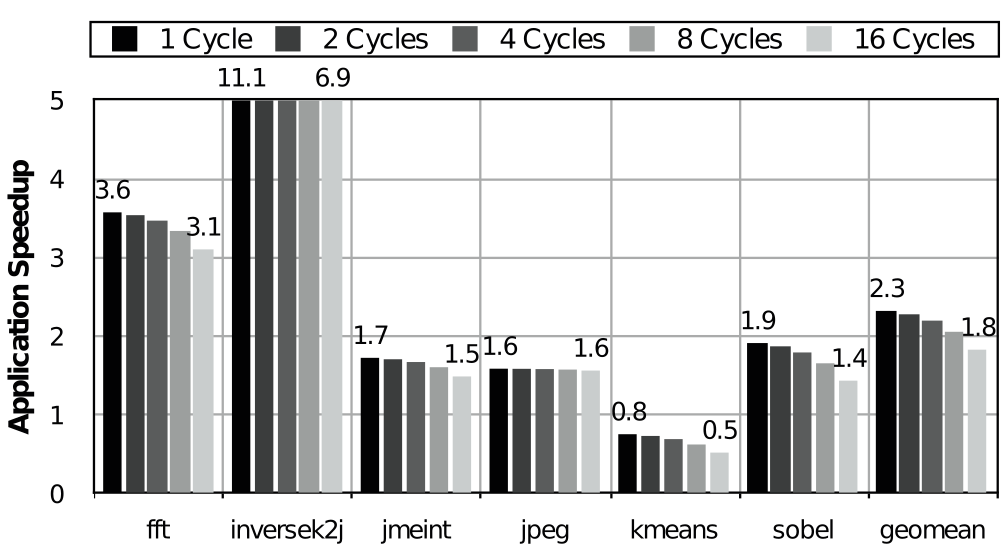
\includegraphics[scale=1.0]{images/fig10.png}\\
        Some applications are more sensitive than others
    }
}

\section{Conclusions}
\frame{
    \frametitle{Food For Thought}
    \begin{itemize}[<+->]
        \item \textbf{Applicability:} Code must be "hot." Approximation must be OK. Inputs and outputs are explicitly defined.
        \item \textbf{Programmer Effort:} Must identify regions of approximable code. Provide the application inputs to be used for training.
        \item \textbf{Quality Control:} \textit{"In other words, without exhaustively exploring the NPU's input space, it is impossible to give guarantees about its worst-case accuracy."}
    \end{itemize}
}

\frame{
    \begin{center}
        \Huge{Questions/Discussion}
    \end{center}
}

\nocite{*} % Include everything in the .bib file.
\bibliographystyle{plainnat}
\bibliography{neural-acceleration}

% that's all, folks
\end{document}
